\documentclass{article}
\usepackage[utf8]{inputenc}

\usepackage{multicol} %Make columns
\usepackage[margin=1in]{geometry} %Change margins
\usepackage[most]{tcolorbox}  % For the "RIT" box on EEEE cover

%%%%% Extra required packages
\usepackage{graphicx}	%provides some extra features for including graphics. 
\usepackage{float}	%Provides the [H] for hard setting things. It means "Put this exactly here
\usepackage[outdir=./]{epstopdf}	%Used to include .eps vector images
\usepackage{caption} %So you can caption things bettr
\usepackage{siunitx} % Formats units and value  s
\usepackage{pgfplotstable} % Generates table from .csv
\usepackage{tocloft} % Adds the ability to format the Table of contensts
\usepackage{csvsimple}
\usepackage{pdfpages}

%edit pdf properties
\usepackage[pdftex,
            pdfauthor=Barry Wu,
            pdftitle=Wu\_Barry\_Machine\_Intelligence\_HW4,
            pdfsubject=Machine Intelligence HW4,
            pdfkeywords=Homework 4,
            pdfproducer={Latex with hyperref, or other system},
            pdfcreator={pdflatex, or other tool}]{hyperref}

\usepackage{listings}
\usepackage{color}

\definecolor{codegreen}{rgb}{0,0.6,0}
\definecolor{codegray}{rgb}{0.5,0.5,0.5}
\definecolor{codepurple}{rgb}{0.58,0,0.82}
\definecolor{backcolour}{rgb}{0.95,0.95,0.92}
 
\lstdefinestyle{mystyle}{
    backgroundcolor=\color{backcolour},   
    commentstyle=\color{codegreen},
    keywordstyle=\color{blue},
    numberstyle=\tiny\color{codegray},
    stringstyle=\color{codepurple},
    basicstyle=\footnotesize,
    breakatwhitespace=false,         
    breaklines=true,                 
    captionpos=b,                    
    keepspaces=true,                 
    numbers=left,                    
    numbersep=5pt,                  
    showspaces=false,                
    showstringspaces=false,
    showtabs=false,                  
    tabsize=2
}
 
\lstset{style=mystyle}
 
\setlength{\parindent}{0pt} % Don't indent paragraphs

\begin{document}
Barry Wu\\
Machine Intelligence\\
Homework 4\\

\section*{Problem 1}
Below is the new costFunctionLogisticRegression.m where the gradient and the cost is not calculated using a loop.

\lstinputlisting[language=matlab, caption=costFunctionLogisticRegression.m]{costFunctionLogisticRegression.m}

\newpage

\section*{Problem 2}
%% lambda = 0
\subsection*{{$\lambda$}=0}
\lstinputlisting[language=matlab, caption=problem\_2.m, firstline=25, lastline=59]{problem_2.m}

\begin{figure}[H]
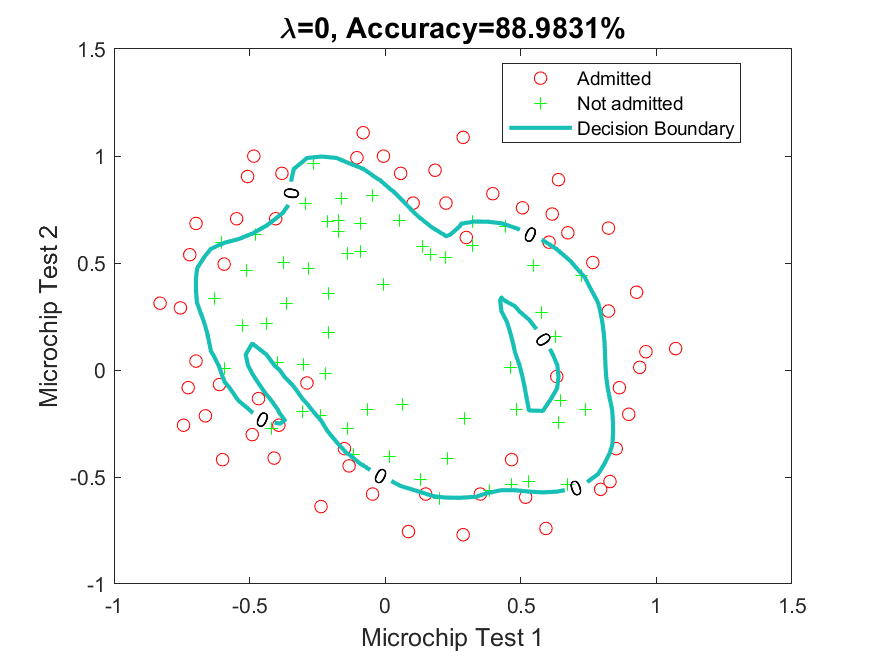
\includegraphics[scale = 0.75]{hwk4_problem2_lambda_0_plot.png}
\end{figure}

%% lambda = 1
\subsection*{{$\lambda$}=1}
\lstinputlisting[language=matlab, caption=problem\_2.m, firstline=61, lastline=95]{problem_2.m}

\begin{figure}[H]
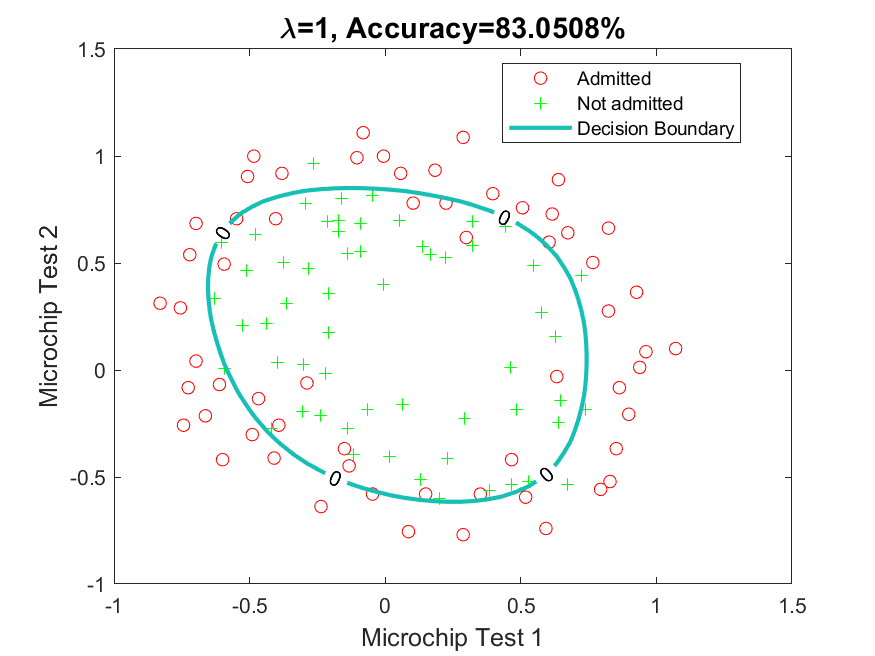
\includegraphics[scale = 0.75]{hwk4_problem2_lambda_1_plot.png}
\end{figure}

%% lambda = 10
\subsection*{{$\lambda$}=10}
\lstinputlisting[language=matlab, caption=problem\_2.m, firstline=97, lastline=131]{problem_2.m}

\begin{figure}[H]
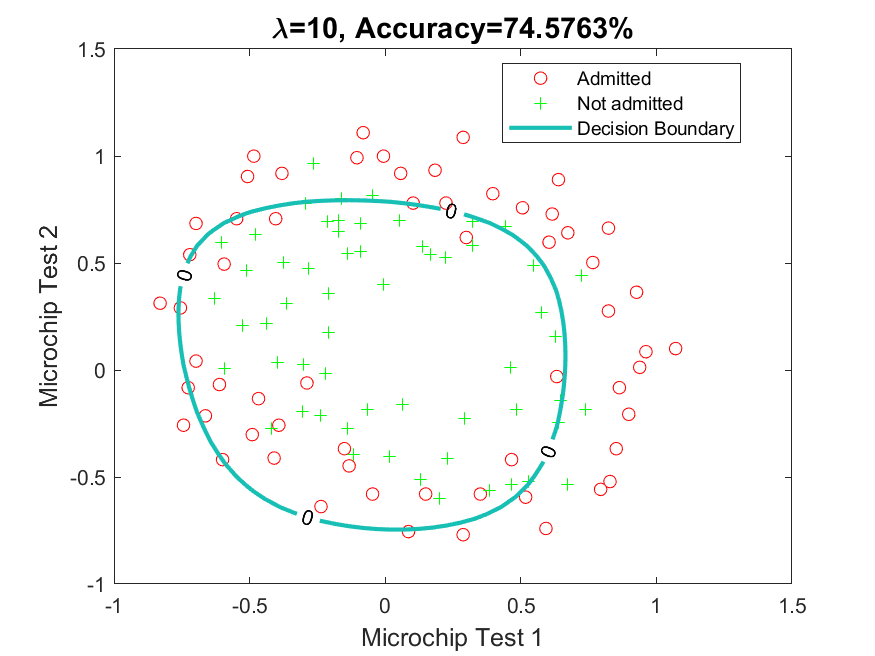
\includegraphics[scale = 0.75]{hwk4_problem2_lambda_10_plot.png}
\end{figure}

%% lambda = 100
\subsection*{{$\lambda$}=100}
\lstinputlisting[language=matlab, caption=problem\_2.m, firstline=133, lastline=167]{problem_2.m}

\begin{figure}[H]
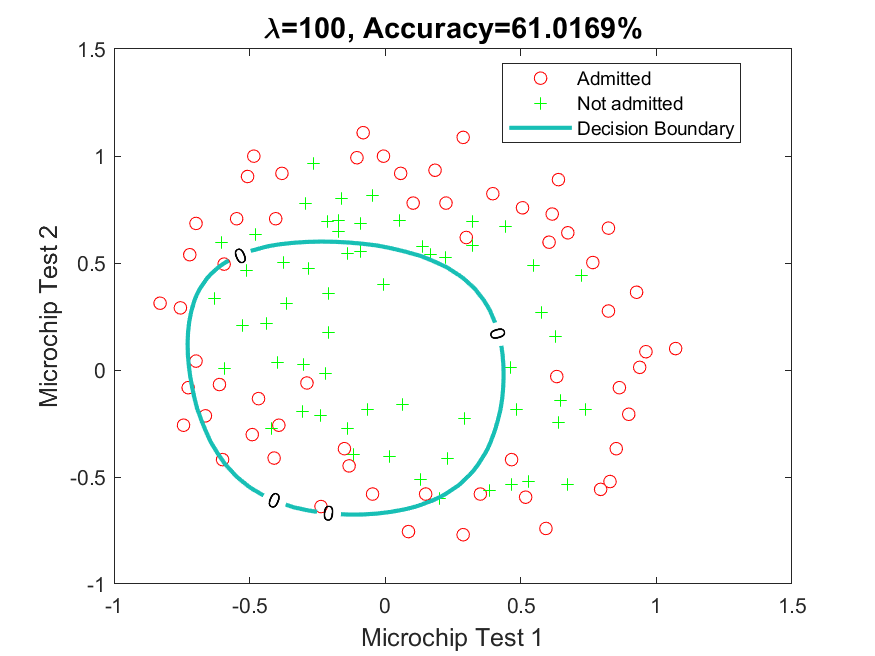
\includegraphics[scale = 0.75]{hwk4_problem2_lambda_100_plot.png}
\end{figure}

\newpage
\section*{Problem 3}
%% lambda = 0
\subsection*{{$\lambda$}=0}
\lstinputlisting[language=matlab, caption=problem\_3.m, firstline=25, lastline=107]{problem_3.m}

\begin{figure}[H]
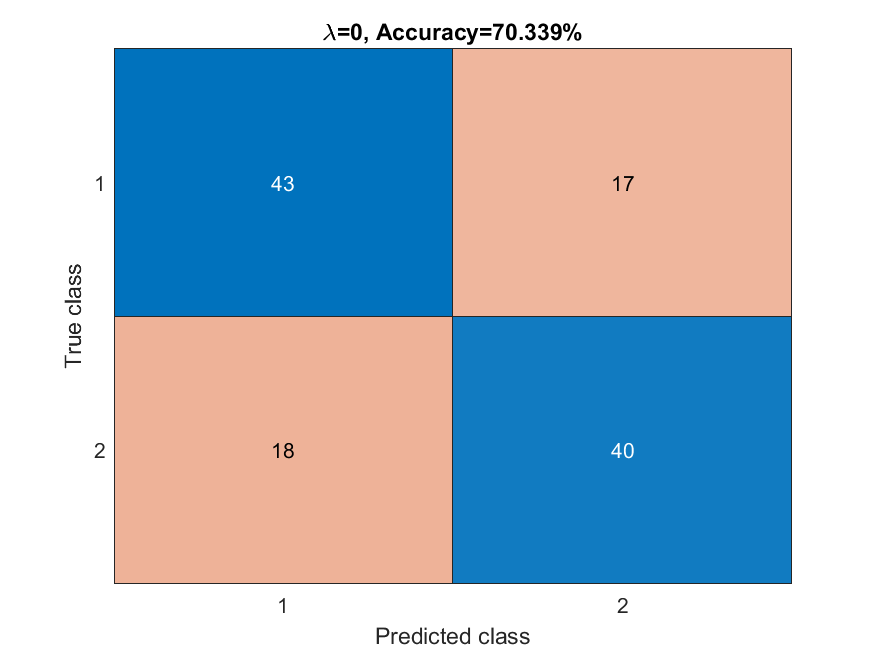
\includegraphics[scale = 0.75]{hwk4_problem3_lambda_0_plot.png}
\end{figure}

%% lambda = 1
\subsection*{{$\lambda$}=1}
\lstinputlisting[language=matlab, caption=problem\_3.m, firstline=117, lastline=200]{problem_3.m}

\begin{figure}[H]
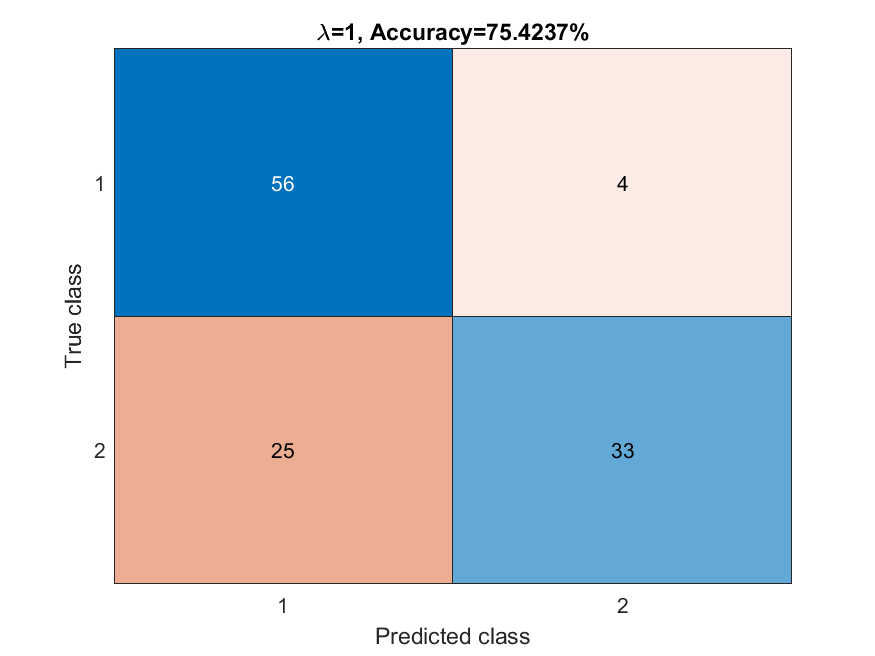
\includegraphics[scale = 0.75]{hwk4_problem3_lambda_1_plot.png}
\end{figure}

%% lambda = 10
\subsection*{{$\lambda$}=10}
\lstinputlisting[language=matlab, caption=problem\_3.m, firstline=210, lastline=293]{problem_3.m}

\begin{figure}[H]
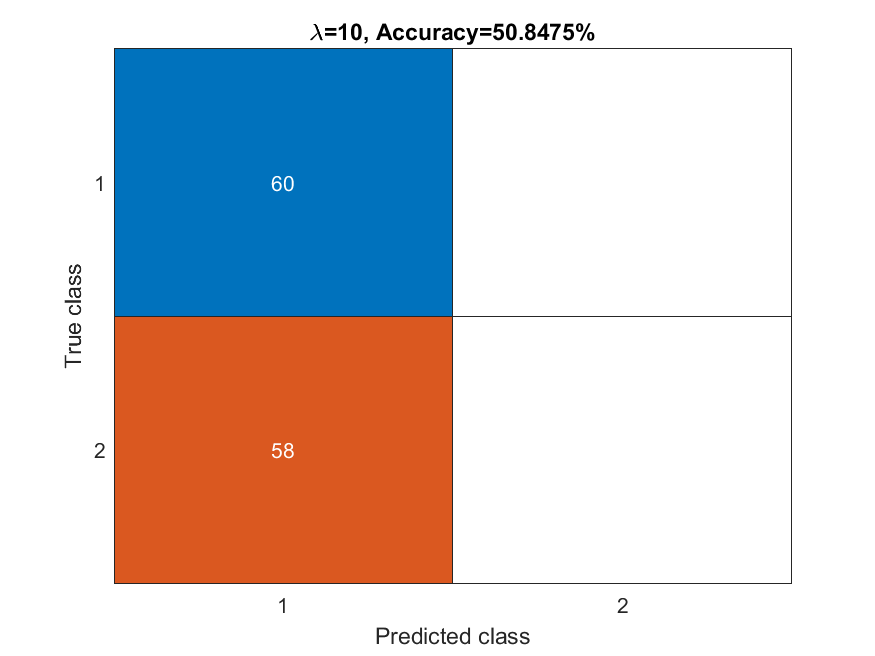
\includegraphics[scale = 0.75]{hwk4_problem3_lambda_10_plot.png}
\end{figure}

%% lambda = 100
\subsection*{{$\lambda$}=100}
\lstinputlisting[language=matlab, caption=problem\_3.m, firstline=304, lastline=387]{problem_3.m}
\begin{figure}[H]
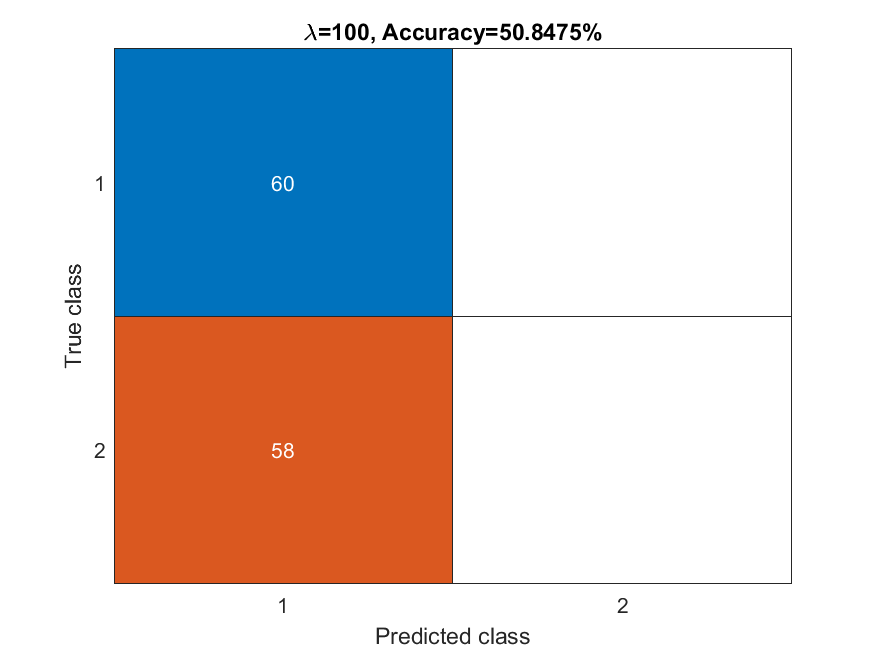
\includegraphics[scale = 0.75]{hwk4_problem3_lambda_100_plot.png}
\end{figure}

\newpage
\section*{Problem 4}
\lstinputlisting[language=matlab, caption=problem\_4.m]{problem_4.m}
\begin{figure}[H]
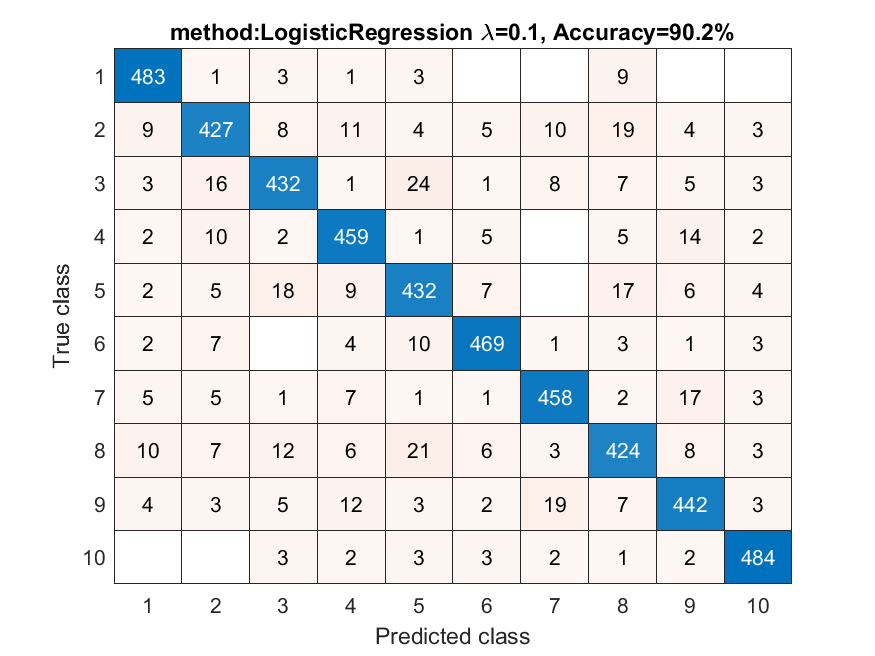
\includegraphics[scale = 0.75]{hwk4_problem4_plot.png}
\end{figure}

\newpage
\section*{Problem 5}
\lstinputlisting[language=matlab, caption=problem\_5.m]{problem_5.m}
\begin{figure}[H]
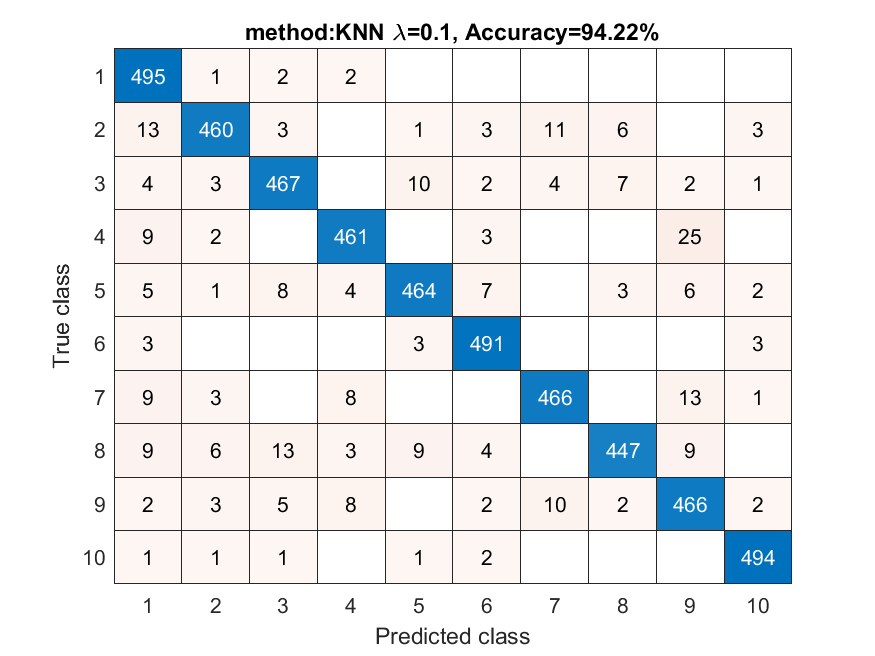
\includegraphics[scale = 0.75]{hwk4_problem5_plot.png}
\end{figure}

%\newpage
%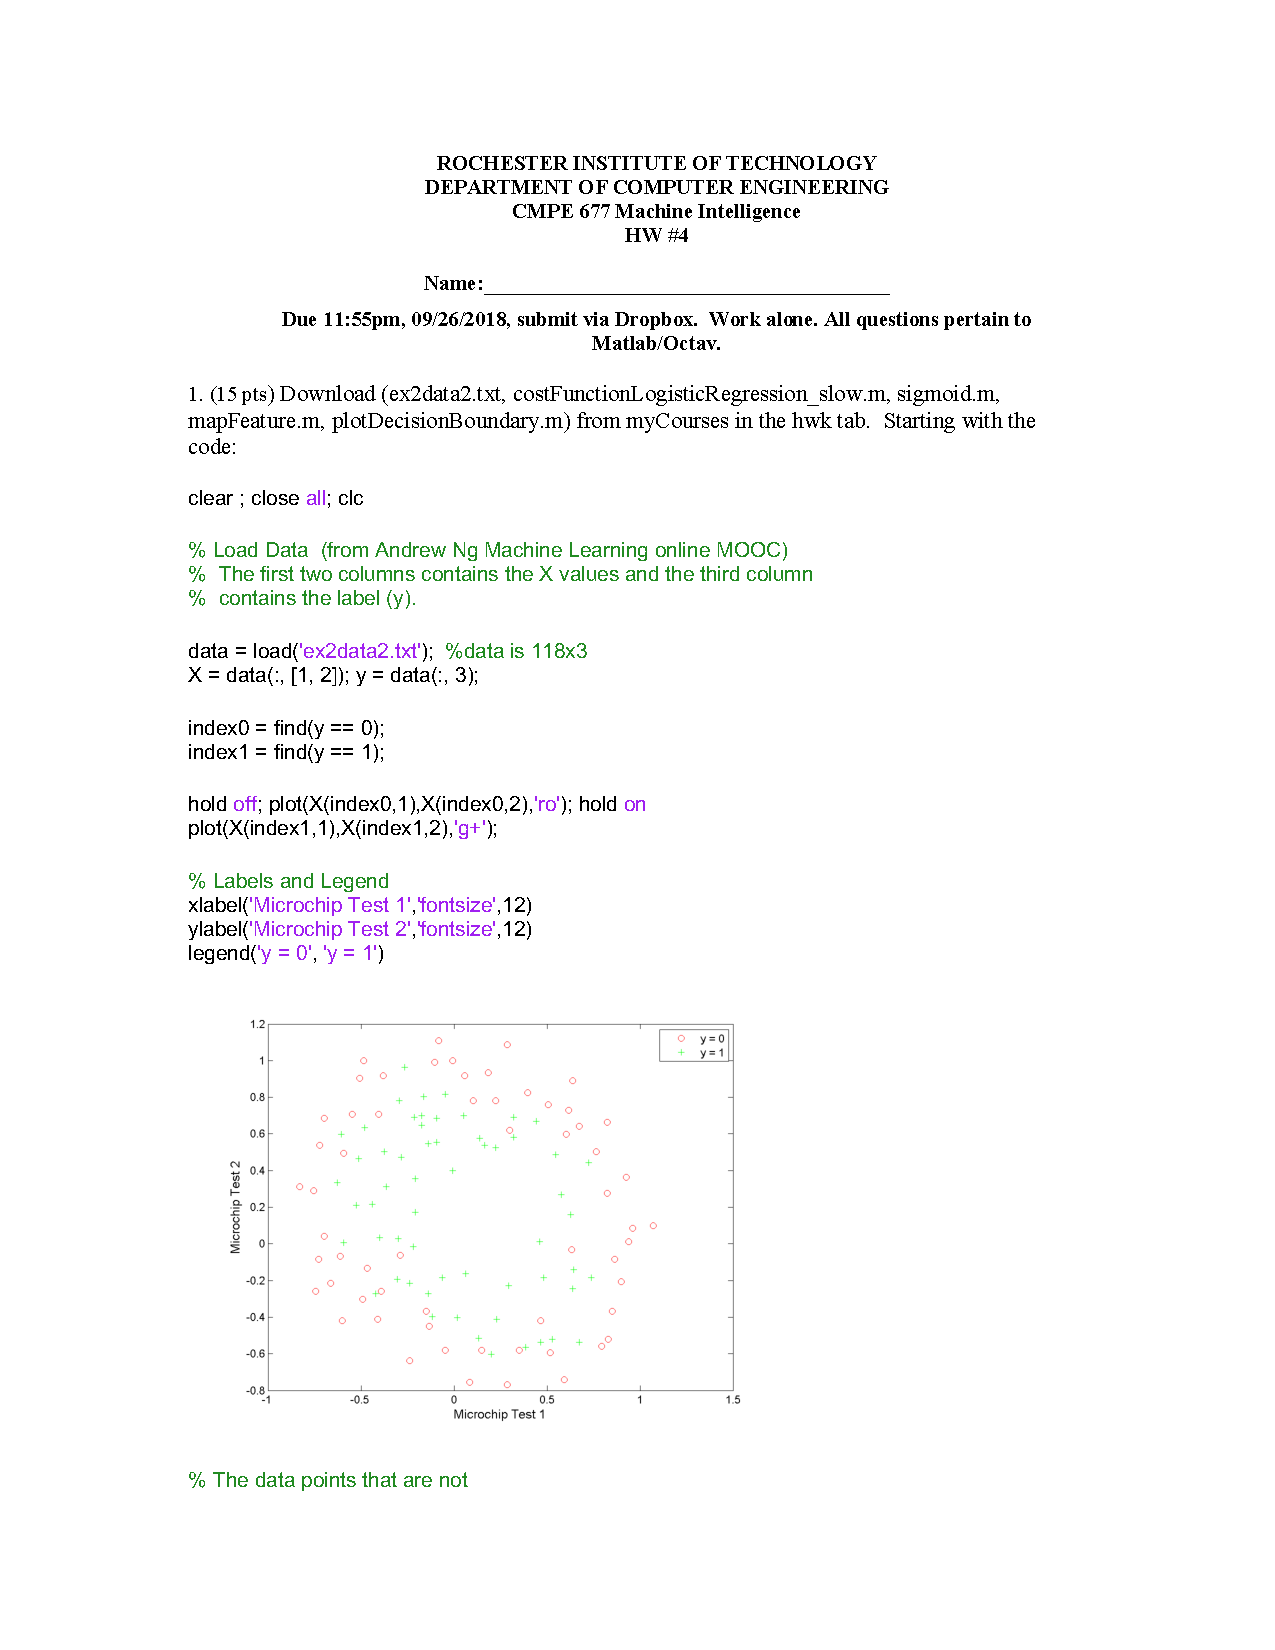
\includepdf[pages=-]{Homework4_CMPE677_2018.pdf}
\end{document}
